\begin{multicols}{2}
\byline{\sc\Large ЗДРАВЕЙ, АЗ}{Чавдар Йорданов, випуск, 1965г.}

\noindent \lettrine[lraise=0.2, nindent=0em, slope=-.5em]{Т}{ази} година се навършват 55 години от създаването на Немската езикова гимназия в 
Бургас. Като се замисля, това са страшно много години. Имах щастието да съм един от първия випуск на гимназията. Аз и моите съученици сега сме 68-годишни. 
Навремето хората на тази възраст ми изглеждаха ужасно стари. И не можех да си представя, че ще доживея до нея. А сега съм точно два пъти по-възрастен от моя баща...
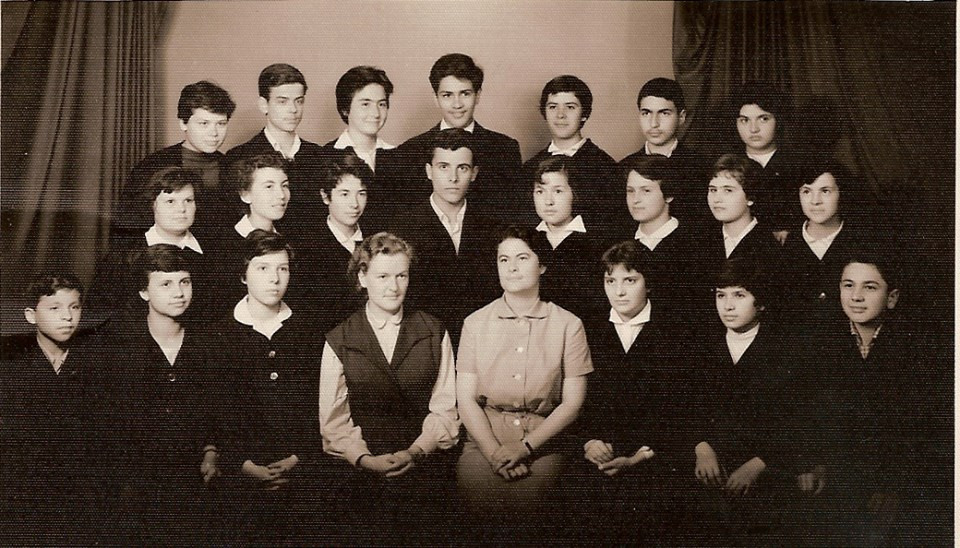
\includegraphics[width=3.4in]{./zdravei_az/2-1.jpg}
Випускът ни беше от 80 човека, от които 50 момичета и 30 момчета, разпределени в 4 класа. Бяхме от Бургас, от Варна, Хасково, Ямбол, Карнобат, Айтос, Пловдив, Сливен, Казанлък, Стара Загора и дори от София. Някъде прочетох, че този първи випуск за изминалите 55 години има най-висок успех в цялата история на гимназията.
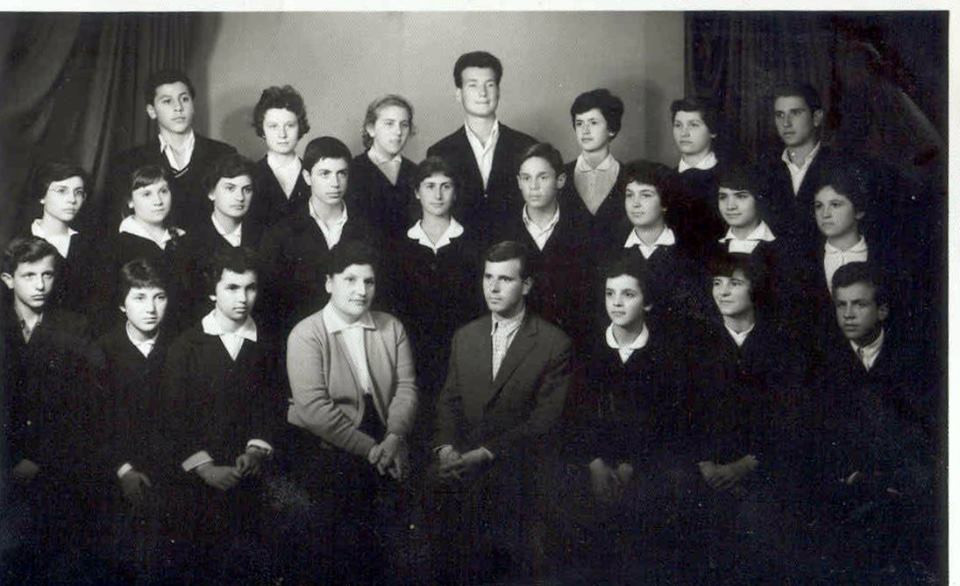
\includegraphics[width=3.4in]{./zdravei_az/2-2.jpg}
От 1995 г. стана традиция ние, първите, да се събираме на всеки 5 години – в Бургас или София. От 15 години живеещите в София се събираме всяка последна сряда на месеца в едно заведение до първата спирка на трамвай No5, като през последните години започваха да идват и съученици от по-малките класове. Имаме чувството, че никога не сме се разделяли. Знаем си всичко за мъжете и жените, за децата и внуците, за болежките и радостите. И постоянно се връщаме към онези – 
първите 5 години...
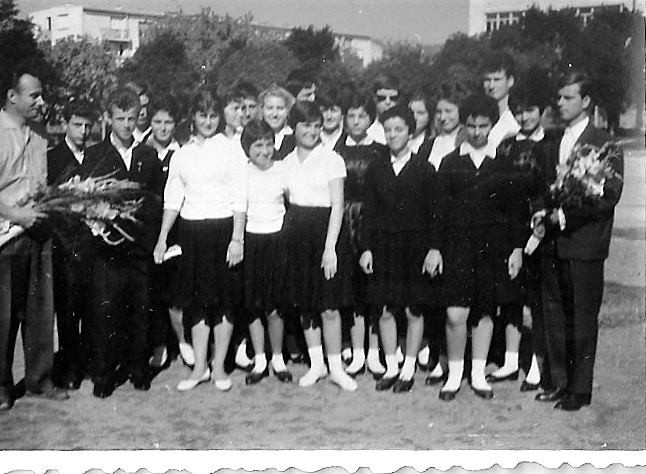
\includegraphics[width=3.4in]{./zdravei_az/2-3.jpg}
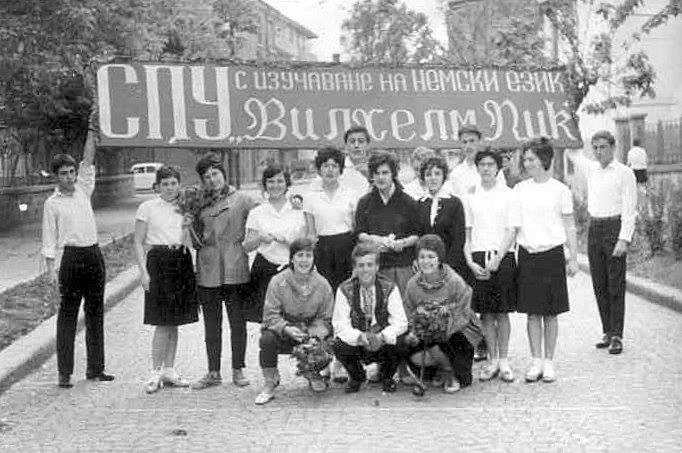
\includegraphics[width=3.4in]{./zdravei_az/2-4.jpg}
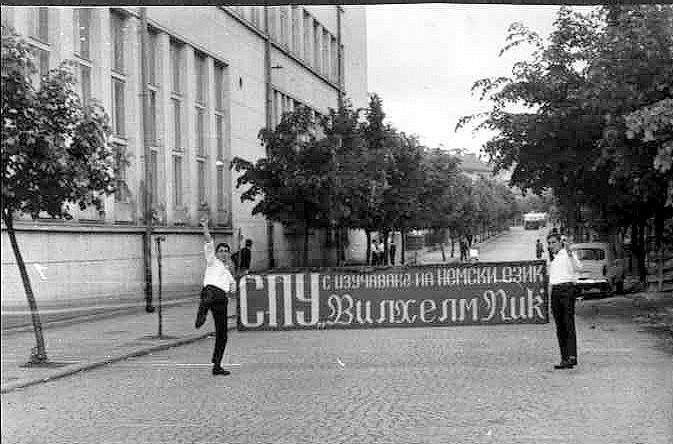
\includegraphics[width=3.4in]{./zdravei_az/2-5.jpg}

\closearticle
\end{multicols}
